\documentclass{article}
\usepackage{tikz}
\usepackage{amsmath}
\usetikzlibrary{matrix}
\title{Connect 4 AI}
\author{David Friedman \and Sridatt Bhamidipati}


\tikzstyle{player} = [circle, minimum size=.4cm, draw=black]
\tikzstyle{threat} = [rectangle, thick, minimum size=.4cm, draw=blue]

\usepackage{subcaption} 
\usepackage{cleveref}

\newcommand{\rd}{\node [player, fill=red]{};}
\newcommand{\yw}{\node [player, fill=yellow] {};}
\newcommand{\gy}{\node [player, fill=white] {};}
\newcommand{\rt}{\node [threat, fill=red!50] {};}
\newcommand{\yt}{\node [threat, fill=yellow!50] {};}
\newcommand{\bt}{\node [threat, fill=orange!50] {};}



\begin{document}
\maketitle
\newpage
\tableofcontents
\newpage

\section{Preface}
This is a project for ECS 170, Artificial Intelligence, at UC Davis. We wrote AI using minimax and alphabeta pruning in order to play and win connect 4.
	
\section{Evaluation}
\subsection{Functions}
Our evaluation function is a combination of two evaluation functions. Before getting into them we must first describe what a winning group is, as we will use this terminology throughout. A winning group is any combination of four slots on the board in one row, column, or diagonal. There are 69 total winning rows in the game. A winning group is owned when only one player has pieces in that group.
\subsubsection{Number owned in winning group}
Our first evaluation function is a a count of all winning groups we own, weighted by the number we own in that group minus the count of all winning groups the opponent owns, again weighted by the number they own in that group. The equation for this is:
\[f_1(x)=\sum_{n \in s_{1,r}}{numOwned_1(n)}-\sum_{n \in s_{2,r}}{numOwned_2(n)}\]
where $numOwned_{r,n}$ represents the number owned by player $r$ in the winning group n, and $s_r$ represents the winning groups soley owned by player $r$.
\subsubsection{Odd/Even Threats}
\label{oddeven}
Our second evaluation function is more complicated. First it iterates over a list of all possible winning groups, and finds the threats. A threat is a slot that would complete a 4 in a row for either team. It then iterates over each of these threats and tallies them, categorizing them based on the team who owns the threat and the threats polarity (odd/even). Even threats are threats that have an even number of (necessarily) empty spaces above them, while odd threats are threats with an odd number of empty spaces above them (figure \ref{threattypes}). The function ignores a threat if there is a threat below it from the opposite team with opposite polarity (the reasoning will be explained in the section \ref{ssec:reasoning}). 
		
The function then checks if player 1 has more odd threats than player 2, if player 2 has two more odd threats than player one, or, if in the case they both have the same number, if player 2 has at least one even threat. If the former is satisfied it returns $100$, signifying that player one is in the lead. For the latter two it returns $-100$, signifying the opposite, and if none of the cases are satisfied we return 0. The equation looks like the following piecewise:
\[ f_2(x,y)=\begin{cases} 
	100 & odd(x)>odd(y) \\
	-100 & odd(y)>odd(x)+1 \\
	-100 & odd(x)=odd(y)~\mbox{and}~even(y) > 0\\
	0 & otherwise
	\end{cases}
\]
where x is all threats by player 1, and y is all threats by player 2.
		
\begin{figure}[t]
	\centering
	\begin{subfigure}[b]{0.4\textwidth}
		\centering
		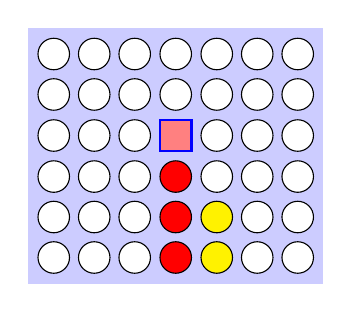
\begin{tikzpicture}
			\fill[blue!20] (0,0) rectangle (3.75,3.25);
			\matrix (mat) at (0,0) [matrix of nodes, ampersand replacement=\&, nodes={circle, minimum size=.4cm},
				anchor= south west,
			column sep={.1cm}, row sep={.1cm}] {
				\gy \& \gy \& \gy \& \gy \& \gy \& \gy \& \gy \\
				\gy \& \gy \& \gy \& \gy \& \gy \& \gy \& \gy \\
				\gy \& \gy \& \gy \& \rt \& \gy \& \gy \& \gy \\
				\gy \& \gy \& \gy \& \rd \& \gy \& \gy \& \gy \\
				\gy \& \gy \& \gy \& \rd \& \yw \& \gy \& \gy \\
				\gy \& \gy \& \gy \& \rd \& \yw \& \gy \& \gy \\
			};
		\end{tikzpicture}
		\caption{Even red threat}
		\label{threatodd}
	\end{subfigure}%
	\begin{subfigure}[b]{0.4\textwidth}
		\centering
		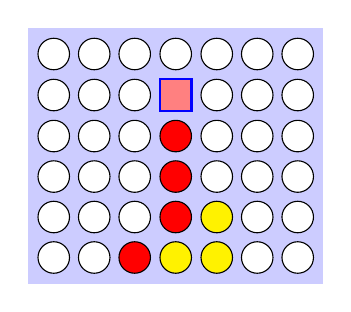
\begin{tikzpicture}
			\fill[blue!20] (0,0) rectangle (3.75,3.25);
			\matrix (mat) at (0,0) [matrix of nodes, ampersand replacement=\&, nodes={circle, minimum size=.4cm},
				anchor= south west,
			column sep={.1cm}, row sep={.1cm}] {
				\gy \& \gy \& \gy \& \gy \& \gy \& \gy \& \gy \\
				\gy \& \gy \& \gy \& \rt \& \gy \& \gy \& \gy \\
				\gy \& \gy \& \gy \& \rd \& \gy \& \gy \& \gy \\
				\gy \& \gy \& \gy \& \rd \& \gy \& \gy \& \gy \\
				\gy \& \gy \& \gy \& \rd \& \yw \& \gy \& \gy \\
				\gy \& \gy \& \rd \& \yw \& \yw \& \gy \& \gy \\
			};
		\end{tikzpicture}
		\caption{Odd red threat}
		\label{threateven}
	\end{subfigure}%
	\caption{Types of threats (threat marked with squares)}
	\label{threattypes}
\end{figure}

\subsubsection{Abandonded function - Islands}
Our last idea for an evaluation function was to count the number of islands created by player 1 and player 2 on the board, compare them, and return a reasonable evaluation value. An island is essentially a connected component in an undirected graph, and we viewed it in a perspective where having more of our same coins clumped together was advantageous to us because we can then make moves from various angles and end up forcing victory over our opponent. Thus, given that the number of player 1's coins and player 2's coins on the board are about the same, having the lesser number of islands could be more advantageous. We solved this by implementing a depth first search, which we would run on each unvisited cell. We proceeded to count up the number of islands for each player. Finally, it was important that we returned the difference of the number of islands rather than the value of the least island count, since we took into consideration that the evaluation should not be extremely high if the difference was small. While it worked sometimes, we quickly found situations where it hurt the evaluation. In addition, we found that the other evaluation functions worked quite well, and decided to stick to those. 

\subsection{Reasoning}
\label{ssec:reasoning}
Our first evaluation function is straightforward. We want to value states where we have more control of the winning positions more. If we control a winning position (only our pieces are in it), we can use it to win. If the enemy controls it they can use it to win. Additionally, if more of our/their pieces are in a winning position, we need less moves to complete that win, which is favourable.
		
Our second evaluation function is more complicated. It relies on the fact that red (player 1) will only ever move when there are an even number of pieces on the board, and yellow (player 2) will only ever move when there are an odd number of pieces on the board. Additionally it relies on the fact that since columns have an even number of slots, red generally has more control over odd positions than even. This is because red plays during all odd turns, and all columns are an even number, meaning once a column has been filled it is generally reds turn again. This means red has an easier time taking odd threats, and yellow has an easier time taking even threats. Therefore, it is logical that red can generally block all of yellows threats and play its own winning threat if it has more of these odd threats. Yellow on the other hand needs to have two more odd threats, as if it only has one more red may use its advantage in playing odd rows to block all these threats before yellow can win. The last case is because if they have an equal number of threats, once red has blocked all of yellows odd threats, yellow will generally have an easier time grabbing an even row, and thus winning with its even threat.
		
As mentionedin setion \ref{oddeven}, we need to be explain \emph{why} we remove threats above another threat if the threat is from the other player and has a different parity. This is quite simple. Take figure \ref{threatblock} as an example. Here orange squares represent threats both players own. Note that yellow's lowest threat is even. However, in order to take it the slot beneath must be filled. Because there are an even number of pieces in play, it is reds turn. Red has an odd threat in the first row. Therefore yellow's even threat may never be taken, as red must play below first and win. Additionally if we for now ignore all but yellows first even threat and reds even threat above it, we can see that the same thing would occur. Therefore in general threats of opposite parity to lower threats by the other player are useless. We can extend this to also mark shared threats by yellow on odd levels as useless for yellow, and shared even threats as useless for red, but we leave this distinction out of our code to keep the runtime of our evaluation fast.
		
\begin{figure}[t]
	\centering
	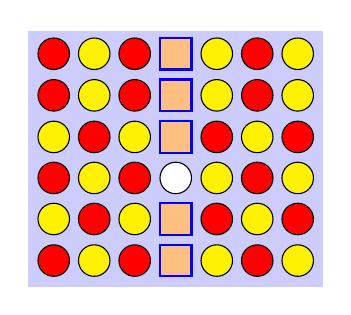
\begin{tikzpicture}
		\fill[blue!20] (0,0) rectangle (3.75,3.25);
		\matrix (mat) at (0,0) [matrix of nodes, ampersand replacement=\&, nodes={circle, minimum size=.4cm},
			anchor= south west,
		column sep={.1cm}, row sep={.1cm}] {
			\rd \& \yw \& \rd \& \bt \& \yw \& \rd \& \yw \\
			\rd \& \yw \& \rd \& \bt \& \yw \& \rd \& \yw \\
			\yw \& \rd \& \yw \& \bt \& \rd \& \yw \& \rd \\
			\rd \& \yw \& \rd \& \gy \& \yw \& \rd \& \yw\ \\
			\yw \& \rd \& \yw \& \bt \& \rd \& \yw \& \rd \\
			\rd \& \yw \& \rd \& \bt \& \yw \& \rd \& \yw \\
		};
	\end{tikzpicture}
	\caption{Useless yellow threat}
	\label{threatblock}
\end{figure}
\subsection{Worked Example}
We will use figure \ref{fig:example} as our example game state. First we will run our second evaluation function, as it is much simpler to run in this case. Threats have been marked their respective team colors. Red has two odd threats, and yellow has one even threat, however one of reds threats is useless because yellow's threat is below it with different parity. However, we still have $odd(x) > odd(y)$, and our evaluation function returns 100.
	
Our second heuristic is a bit lengthier to run through, as there are a total of 69 winning positions we need to consider. Here, however, only 8 winning positions are not invalid due to having two different players in them, and of those two (the rightmost column starting from the top and the second from top) have no pieces in them. We can easily count the number owned by red and yellow in each group, and we see that the result is $7-6 = 1$.

Both our evaluation functions favour red, and as seen in figure \ref{fig:win}, we have guessed correctly as red does win.
\begin{figure}[t]
	\centering
	\begin{subfigure}[b]{0.4\textwidth}
		\centering
		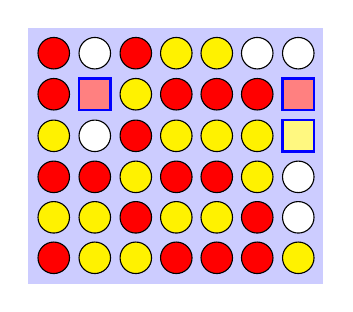
\begin{tikzpicture}
			\fill[blue!20] (0,0) rectangle (3.75,3.25);
			\matrix (mat) at (0,0) [matrix of nodes, ampersand replacement=\&, nodes={circle, minimum size=.4cm},
				anchor= south west,
			column sep={.1cm}, row sep={.1cm}] {
				\rd \& \gy \& \rd \& \yw \& \yw \& \gy \& \gy \\
				\rd \& \rt \& \yw \& \rd \& \rd \& \rd \& \rt \\
				\yw \& \gy \& \rd \& \yw \& \yw \& \yw \& \yt \\
				\rd \& \rd \& \yw \& \rd \& \rd \& \yw \& \gy \\
				\yw \& \yw \& \rd \& \yw \& \yw \& \rd \& \gy \\
				\rd \& \yw \& \yw \& \rd \& \rd \& \rd \& \yw \\
			};
		\end{tikzpicture}
		\caption{Red to win}
		\label{fig:example}
	\end{subfigure}
	\begin{subfigure}[b]{0.4\textwidth}
		\centering
		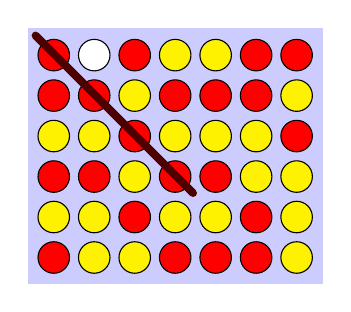
\begin{tikzpicture}
			\fill[blue!20] (0,0) rectangle (3.75,3.25);
			\matrix (mat) at (0,0) [matrix of nodes, ampersand replacement=\&, nodes={circle, minimum size=.4cm},
				anchor= south west,
			column sep={.1cm}, row sep={.1cm}] {
				\rd \& \gy \& \rd \& \yw \& \yw \& \rd \& \rd \\
				\rd \& \rd \& \yw \& \rd \& \rd \& \rd \& \yw \\
				\yw \& \yw \& \rd \& \yw \& \yw \& \yw \& \rd \\
				\rd \& \rd \& \yw \& \rd \& \rd \& \yw \& \yw \\
				\yw \& \yw \& \rd \& \yw \& \yw \& \rd \& \yw \\
				\rd \& \yw \& \yw \& \rd \& \rd \& \rd \& \yw \\
			};
			\draw[line width=.1cm, draw=red!30!black, cap=round] (.1,3.15) -- (2.1, 1.15);
		\end{tikzpicture}
		\caption{Red wins}
		\label{fig:win}
	\end{subfigure}
	\caption{Example}
\end{figure}
\newpage
\section{MiniMax Against poor AI}
We win every game in the section below. We played around half of the games as player one, and around half of the games as player two (Our player is indicated below each board).
\subsection{Against StupidAI}
\begin{figure}[h]
	\centering
	\begin{subfigure}[b]{0.4\textwidth}
		\centering
		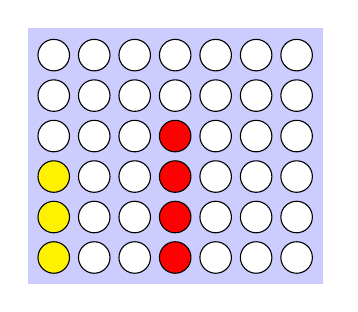
\begin{tikzpicture}
			\fill[blue!20] (0,0) rectangle (3.75,3.25);
			\matrix (mat) at (0,0) [matrix of nodes, ampersand replacement=\&, nodes={circle, minimum size=.4cm},
				anchor= south west,
			column sep={.1cm}, row sep={.1cm}] {
				\gy \& \gy \& \gy \& \gy \& \gy \& \gy \& \gy \& \\
				\gy \& \gy \& \gy \& \gy \& \gy \& \gy \& \gy \& \\
				\gy \& \gy \& \gy \& \rd \& \gy \& \gy \& \gy \& \\
				\yw \& \gy \& \gy \& \rd \& \gy \& \gy \& \gy \& \\
				\yw \& \gy \& \gy \& \rd \& \gy \& \gy \& \gy \& \\
				\yw \& \gy \& \gy \& \rd \& \gy \& \gy \& \gy \& \\
			};
			%\draw[line width=.1cm, draw=red!30!black, cap=round] (1.87,2.10) -- (1.87, 0.10);
		\end{tikzpicture}
		\caption{As player 1}
		\label{fig:stup1}
	\end{subfigure}
	\begin{subfigure}[b]{0.4\textwidth}
		\centering
		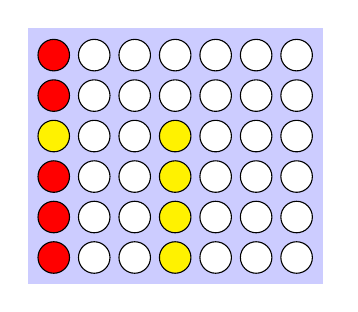
\begin{tikzpicture}
			\fill[blue!20] (0,0) rectangle (3.75,3.25);
			\matrix (mat) at (0,0) [matrix of nodes, ampersand replacement=\&, nodes={circle, minimum size=.4cm},
				anchor= south west,
			column sep={.1cm}, row sep={.1cm}] {
				\rd \& \gy \& \gy \& \gy \& \gy \& \gy \& \gy \& \\
				\rd \& \gy \& \gy \& \gy \& \gy \& \gy \& \gy \& \\
				\yw \& \gy \& \gy \&  \yw \& \gy \& \gy \& \gy \& \\
				\rd \& \gy \& \gy \&  \yw \& \gy \& \gy \& \gy \& \\
				\rd \& \gy \& \gy \&  \yw \& \gy \& \gy \& \gy \& \\
				\rd \& \gy \& \gy \&  \yw \& \gy \& \gy \& \gy \& \\
			};
			%\draw[line width=.1cm, draw=yellow!30!black, cap=round] (1.87,2.10) -- (1.87, 0.10);
		\end{tikzpicture}
		\caption{As player 2}
		\label{fig:stup2}
	\end{subfigure}
\end{figure}
	
If MiniMax goes first see \ref{fig:stup1} otherwise see \ref{fig:stup2}. Games depend only on who goes first (we use no randomness so seed has no effect, last three game plays identical so omitted for brevity). We win all 5 games.
	
\newpage
\subsection{Against RandomAI}
Against the random AI we win all 5 games, both as player 1 and as player 2.
\begin{figure}[ht]
	\centering
	\begin{subfigure}[b]{0.4\linewidth}%
		\centering%
		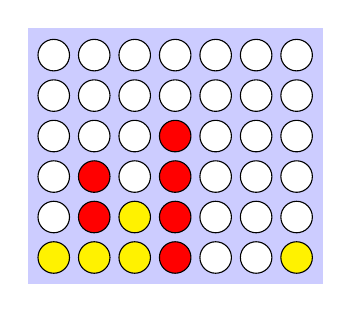
\begin{tikzpicture}%
			\fill[blue!20] (0,0) rectangle (3.75,3.25);
			\matrix (mat) at (0,0) [matrix of nodes, ampersand replacement=\&, nodes={circle, minimum size=.4cm},
				anchor= south west,
			column sep={.1cm}, row sep={.1cm}] { \gy \&  \gy \&  \gy \&  \gy \&  \gy \&  \gy \&  \gy \&  \\
				\gy \&  \gy \&  \gy \&  \gy \&  \gy \&  \gy \&  \gy \&  \\
				\gy \&  \gy \&  \gy \&  \rd \&  \gy \&  \gy \&  \gy \&  \\
				\gy \&  \rd \&  \gy \&  \rd \&  \gy \&  \gy \&  \gy \&  \\
				\gy \&  \rd \&  \yw \& \rd \&  \gy \&  \gy \&  \gy \&  \\
				\yw \& \yw \& \yw \& \rd \&  \gy \&  \gy \&  \yw \& \\
			};
			%\draw[line width=.1cm, draw=red!30!black, cap=round] (1.87,2.10) -- (1.87, 0.10);
		\end{tikzpicture}%
		\caption{As player 1}%
		\label{fig:ran2}%
	\end{subfigure}%
	\begin{subfigure}[b]{0.4\linewidth}%
		\centering%
		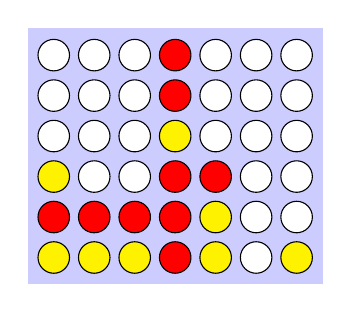
\begin{tikzpicture}%
			\fill[blue!20] (0,0) rectangle (3.75,3.25);
			\matrix (mat) at (0,0) [matrix of nodes, ampersand replacement=\&, nodes={circle, minimum size=.4cm},
				anchor= south west,
			column sep={.1cm}, row sep={.1cm}] { \gy \&  \gy \&  \gy \&  \rd \&  \gy \&  \gy \&  \gy \&  \\
				\gy \&  \gy \&  \gy \&  \rd \&  \gy \&  \gy \&  \gy \&  \\
				\gy \&  \gy \&  \gy \&  \yw \& \gy \&  \gy \&  \gy \&  \\
				\yw \& \gy \&  \gy \&  \rd \&  \rd \&  \gy \&  \gy \&  \\
				\rd \&  \rd \&  \rd \&  \rd \&  \yw \& \gy \&  \gy \&  \\
				\yw \& \yw \& \yw \& \rd \&  \yw \& \gy \&  \yw \& \\
			};
		\end{tikzpicture}%
		\caption{As player 1}%
		\label{fig:ran2}%
	\end{subfigure}%
	
	\begin{subfigure}[b]{0.4\linewidth}%
		\centering%
		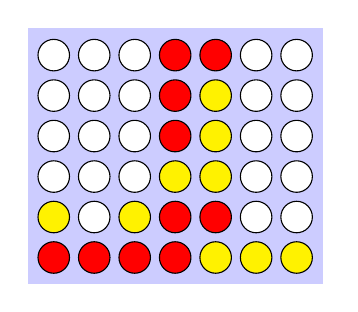
\begin{tikzpicture}%
			\fill[blue!20] (0,0) rectangle (3.75,3.25);
			\matrix (mat) at (0,0) [matrix of nodes, ampersand replacement=\&, nodes={circle, minimum size=.4cm},
				anchor= south west,
			column sep={.1cm}, row sep={.1cm}] { \gy \&  \gy \&  \gy \&  \rd \&  \rd \&  \gy \&  \gy \&  \\
				\gy \&  \gy \&  \gy \&  \rd \&  \yw \& \gy \&  \gy \&  \\
				\gy \&  \gy \&  \gy \&  \rd \&  \yw \& \gy \&  \gy \&  \\
				\gy \&  \gy \&  \gy \&  \yw \& \yw \& \gy \&  \gy \&  \\
				\yw \& \gy \&  \yw \& \rd \&  \rd \&  \gy \&  \gy \&  \\
				\rd \&  \rd \&  \rd \&  \rd \&  \yw \& \yw \& \yw \& \\
			};
		\end{tikzpicture}%
		\caption{As player 1}%
		\label{fig:ran2}%
	\end{subfigure}%
	\begin{subfigure}[b]{0.4\linewidth}%
		\centering%
		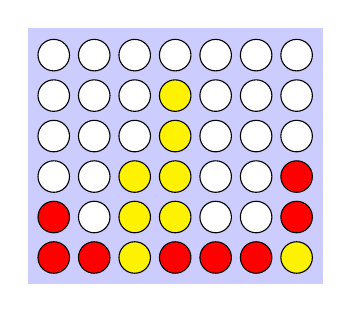
\begin{tikzpicture}%
			\fill[blue!20] (0,0) rectangle (3.75,3.25);
			\matrix (mat) at (0,0) [matrix of nodes, ampersand replacement=\&, nodes={circle, minimum size=.4cm},
				anchor= south west,
			column sep={.1cm}, row sep={.1cm}] { \gy \&  \gy \&  \gy \&  \gy \&  \gy \&  \gy \&  \gy \&  \\
				\gy \&  \gy \&  \gy \&  \yw \& \gy \&  \gy \&  \gy \&  \\
				\gy \&  \gy \&  \gy \&  \yw \& \gy \&  \gy \&  \gy \&  \\
				\gy \&  \gy \&  \yw \& \yw \& \gy \&  \gy \&  \rd \&  \\
				\rd \&  \gy \&  \yw \& \yw \& \gy \&  \gy \&  \rd \&  \\
				\rd \&  \rd \&  \yw \& \rd \&  \rd \&  \rd \&  \yw \& \\
			};
			%\draw[line width=.1cm, draw=yellow!30!black, cap=round] (1.87,2.60) -- (1.87, 0.6);
		\end{tikzpicture}%
		\caption{As player 2}%
		\label{fig:ran2}%
	\end{subfigure}
	
	\begin{subfigure}[b]{0.4\linewidth}%
		\centering%
		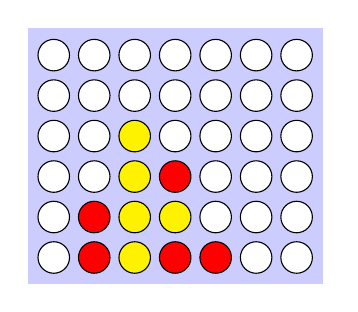
\begin{tikzpicture}%
			\fill[blue!20] (0,0) rectangle (3.75,3.25);
			\matrix (mat) at (0,0) [matrix of nodes, ampersand replacement=\&, nodes={circle, minimum size=.4cm},
				anchor= south west,
			column sep={.1cm}, row sep={.1cm}] { \gy \&  \gy \&  \gy \&  \gy \&  \gy \&  \gy \&  \gy \&  \\
				\gy \&  \gy \&  \gy \&  \gy \&  \gy \&  \gy \&  \gy \&  \\
				\gy \&  \gy \&  \yw \& \gy \&  \gy \&  \gy \&  \gy \&  \\
				\gy \&  \gy \&  \yw \& \rd \&  \gy \&  \gy \&  \gy \&  \\
				\gy \&  \rd \&  \yw \& \yw \& \gy \&  \gy \&  \gy \&  \\
				\gy \&  \rd \&  \yw \& \rd \&  \rd \&  \gy \&  \gy \&  \\
			};
		\end{tikzpicture}%
		\caption{As player 2}%
		\label{fig:ran2}%
	\end{subfigure}%
	%
\end{figure}%
\newpage
\subsection{Against MonteCarloAI}
Against Monte Carlo AI we win every game. Shown below are 10 games against MonteCarloAI, half as player 1 and half as player 2. We win all 10 games.
\begin{figure}[!ht]%
	\centering
	\begin{subfigure}[b]{0.35\textwidth}%
		\centering%
		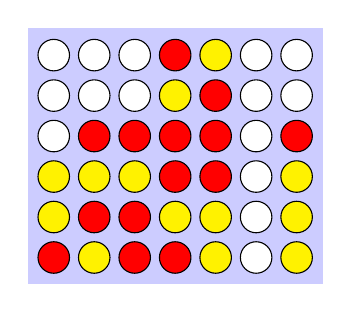
\begin{tikzpicture}%
			\fill[blue!20] (0,0) rectangle (3.75,3.25);%
			\matrix (mat) at (0,0) [matrix of nodes, ampersand replacement=\&, nodes={circle, minimum size=.4cm},%
				anchor= south west,%
			column sep={.1cm}, row sep={.1cm}] { \gy \&  \gy \&  \gy \&  \rd \&  \yw \& \gy \&  \gy \&  \\%
				\gy \&  \gy \&  \gy \&  \yw \& \rd \&  \gy \&  \gy \&  \\%
				\gy \&  \rd \&  \rd \&  \rd \&  \rd \&  \gy \&  \rd \&  \\%
				\yw \& \yw \& \yw \& \rd \&  \rd \&  \gy \&  \yw \& \\%
				\yw \& \rd \&  \rd \&  \yw \& \yw \& \gy \&  \yw \& \\%
				\rd \&  \yw \& \rd \&  \rd \&  \yw \& \gy \&  \yw \& \\%
			};%
		\end{tikzpicture}%
		\caption{As player 1}%
		\label{fig:monty}%
	\end{subfigure}%
	%
	\begin{subfigure}[b]{0.35\textwidth}%
		\centering%
		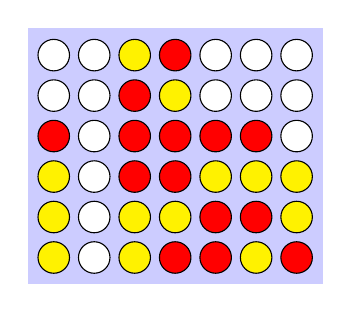
\begin{tikzpicture}%
			\fill[blue!20] (0,0) rectangle (3.75,3.25);%
			\matrix (mat) at (0,0) [matrix of nodes, ampersand replacement=\&, nodes={circle, minimum size=.4cm},%
				anchor= south west,%
			column sep={.1cm}, row sep={.1cm}] { \gy \&  \gy \&  \yw \& \rd \&  \gy \&  \gy \&  \gy \&  \\%
				\gy \&  \gy \&  \rd \&  \yw \& \gy \&  \gy \&  \gy \&  \\%
				\rd \&  \gy \&  \rd \&  \rd \&  \rd \&  \rd \&  \gy \&  \\%
				\yw \& \gy \&  \rd \&  \rd \&  \yw \& \yw \& \yw \& \\%
				\yw \& \gy \&  \yw \& \yw \& \rd \&  \rd \&  \yw \& \\%
				\yw \& \gy \&  \yw \& \rd \&  \rd \&  \yw \& \rd \&  \\%
			};%
		\end{tikzpicture}%
		\caption{As player 1}%
		\label{fig:monty}%
	\end{subfigure}%
	\begin{subfigure}[b]{0.35\textwidth}%
		\centering%
		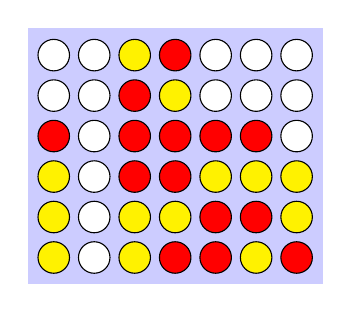
\begin{tikzpicture}%
			\fill[blue!20] (0,0) rectangle (3.75,3.25);%
			\matrix (mat) at (0,0) [matrix of nodes, ampersand replacement=\&, nodes={circle, minimum size=.4cm},%
				anchor= south west,%
			column sep={.1cm}, row sep={.1cm}] { \gy \&  \gy \&  \yw \& \rd \&  \gy \&  \gy \&  \gy \&  \\%
				\gy \&  \gy \&  \rd \&  \yw \& \gy \&  \gy \&  \gy \&  \\%
				\rd \&  \gy \&  \rd \&  \rd \&  \rd \&  \rd \&  \gy \&  \\%
				\yw \& \gy \&  \rd \&  \rd \&  \yw \& \yw \& \yw \& \\%
				\yw \& \gy \&  \yw \& \yw \& \rd \&  \rd \&  \yw \& \\%
				\yw \& \gy \&  \yw \& \rd \&  \rd \&  \yw \& \rd \&  \\%
			};%
		\end{tikzpicture}%
		\caption{As player 1}%
		\label{fig:monty}%
	\end{subfigure}%
	
	\begin{subfigure}[b]{0.35\textwidth}%
		\centering%
		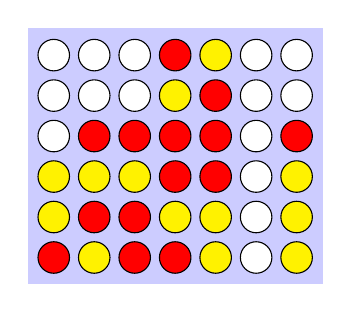
\begin{tikzpicture}%
			\fill[blue!20] (0,0) rectangle (3.75,3.25);%
			\matrix (mat) at (0,0) [matrix of nodes, ampersand replacement=\&, nodes={circle, minimum size=.4cm},%
				anchor= south west,%
			column sep={.1cm}, row sep={.1cm}] { \gy \&  \gy \&  \gy \&  \rd \&  \yw \& \gy \&  \gy \&  \\%
				\gy \&  \gy \&  \gy \&  \yw \& \rd \&  \gy \&  \gy \&  \\%
				\gy \&  \rd \&  \rd \&  \rd \&  \rd \&  \gy \&  \rd \&  \\%
				\yw \& \yw \& \yw \& \rd \&  \rd \&  \gy \&  \yw \& \\%
				\yw \& \rd \&  \rd \&  \yw \& \yw \& \gy \&  \yw \& \\%
				\rd \&  \yw \& \rd \&  \rd \&  \yw \& \gy \&  \yw \& \\%
			};%
		\end{tikzpicture}%
		\caption{As player 1}%
		\label{fig:monty}%
	\end{subfigure}%
	\begin{subfigure}[b]{0.35\textwidth}%
		\centering%
		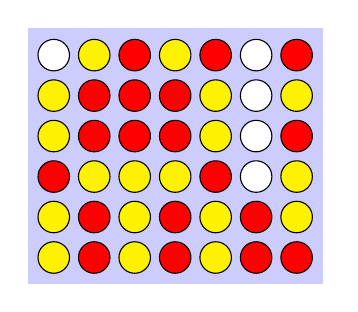
\begin{tikzpicture}%
			\fill[blue!20] (0,0) rectangle (3.75,3.25);%
			\matrix (mat) at (0,0) [matrix of nodes, ampersand replacement=\&, nodes={circle, minimum size=.4cm},%
				anchor= south west,%
			column sep={.1cm}, row sep={.1cm}] { \gy \&  \yw \& \rd \&  \yw \& \rd \&  \gy \&  \rd \&  \\%
				\yw \& \rd \&  \rd \&  \rd \&  \yw \& \gy \&  \yw \& \\%
				\yw \& \rd \&  \rd \&  \rd \&  \yw \& \gy \&  \rd \&  \\%
				\rd \&  \yw \& \yw \& \yw \& \rd \&  \gy \&  \yw \& \\%
				\yw \& \rd \&  \yw \& \rd \&  \yw \& \rd \&  \yw \& \\%
				\yw \& \rd \&  \yw \& \rd \&  \yw \& \rd \&  \rd \&  \\%
			};%
		\end{tikzpicture}%
		\caption{As player 1}%
		\label{fig:monty}%
	\end{subfigure}%
	%
	\begin{subfigure}[b]{0.35\textwidth}%
		\centering%
		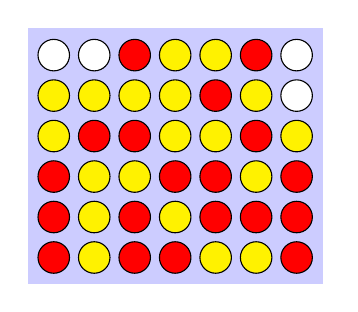
\begin{tikzpicture}%
			\fill[blue!20] (0,0) rectangle (3.75,3.25);%
			\matrix (mat) at (0,0) [matrix of nodes, ampersand replacement=\&, nodes={circle, minimum size=.4cm},%
				anchor= south west,%
			column sep={.1cm}, row sep={.1cm}] { \gy \&  \gy \&  \rd \&  \yw \& \yw \& \rd \&  \gy \&  \\%
				\yw \& \yw \& \yw \& \yw \& \rd \&  \yw \& \gy \&  \\%
				\yw \& \rd \&  \rd \&  \yw \& \yw \& \rd \&  \yw \& \\%
				\rd \&  \yw \& \yw \& \rd \&  \rd \&  \yw \& \rd \&  \\%
				\rd \&  \yw \& \rd \&  \yw \& \rd \&  \rd \&  \rd \&  \\%
				\rd \&  \yw \& \rd \&  \rd \&  \yw \& \yw \& \rd \&  \\%
			};%
		\end{tikzpicture}%
		\caption{As player 2}%
		\label{fig:monty}%
	\end{subfigure}%
		
	\begin{subfigure}[b]{0.35\textwidth}%
		\centering%
		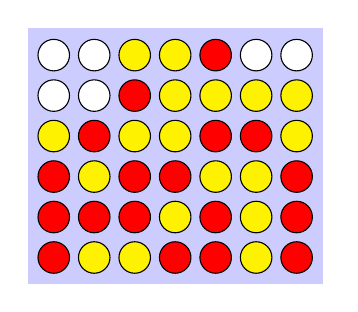
\begin{tikzpicture}%
			\fill[blue!20] (0,0) rectangle (3.75,3.25);%
			\matrix (mat) at (0,0) [matrix of nodes, ampersand replacement=\&, nodes={circle, minimum size=.4cm},%
				anchor= south west,%
			column sep={.1cm}, row sep={.1cm}] { \gy \&  \gy \&  \yw \& \yw \& \rd \&  \gy \&  \gy \&  \\%
				\gy \&  \gy \&  \rd \&  \yw \& \yw \& \yw \& \yw \& \\%
				\yw \& \rd \&  \yw \& \yw \& \rd \&  \rd \&  \yw \& \\%
				\rd \&  \yw \& \rd \&  \rd \&  \yw \& \yw \& \rd \&  \\%
				\rd \&  \rd \&  \rd \&  \yw \& \rd \&  \yw \& \rd \&  \\%
				\rd \&  \yw \& \yw \& \rd \&  \rd \&  \yw \& \rd \&  \\%
			};%
		\end{tikzpicture}%
		\caption{As player 2}%
		\label{fig:monty}%
	\end{subfigure}%
	\begin{subfigure}[b]{0.35\textwidth}%
		\centering%
		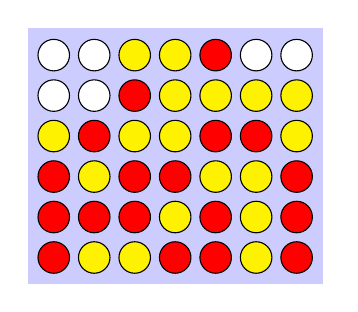
\begin{tikzpicture}%
			\fill[blue!20] (0,0) rectangle (3.75,3.25);%
			\matrix (mat) at (0,0) [matrix of nodes, ampersand replacement=\&, nodes={circle, minimum size=.4cm},%
				anchor= south west,%
			column sep={.1cm}, row sep={.1cm}] { \gy \&  \gy \&  \yw \& \yw \& \rd \&  \gy \&  \gy \&  \\%
				\gy \&  \gy \&  \rd \&  \yw \& \yw \& \yw \& \yw \& \\%
				\yw \& \rd \&  \yw \& \yw \& \rd \&  \rd \&  \yw \& \\%
				\rd \&  \yw \& \rd \&  \rd \&  \yw \& \yw \& \rd \&  \\%
				\rd \&  \rd \&  \rd \&  \yw \& \rd \&  \yw \& \rd \&  \\%
				\rd \&  \yw \& \yw \& \rd \&  \rd \&  \yw \& \rd \&  \\%
			};%
		\end{tikzpicture}%
		\caption{As player 2}%
		\label{fig:monty}%
	\end{subfigure}%
	\begin{subfigure}[b]{0.35\textwidth}%
		\centering%
		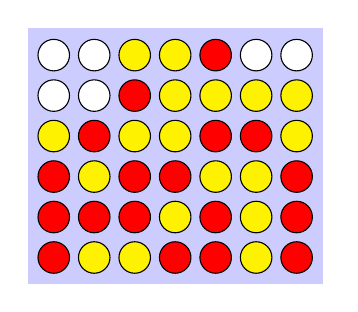
\begin{tikzpicture}%
			\fill[blue!20] (0,0) rectangle (3.75,3.25);%
			\matrix (mat) at (0,0) [matrix of nodes, ampersand replacement=\&, nodes={circle, minimum size=.4cm},%
				anchor= south west,%
			column sep={.1cm}, row sep={.1cm}] { \gy \&  \gy \&  \yw \& \yw \& \rd \&  \gy \&  \gy \&  \\%
				\gy \&  \gy \&  \rd \&  \yw \& \yw \& \yw \& \yw \& \\
				\yw \& \rd \&  \yw \& \yw \& \rd \&  \rd \&  \yw \& \\
				\rd \&  \yw \& \rd \&  \rd \&  \yw \& \yw \& \rd \&  \\
				\rd \&  \rd \&  \rd \&  \yw \& \rd \&  \yw \& \rd \&  \\
				\rd \&  \yw \& \yw \& \rd \&  \rd \&  \yw \& \rd \&  \\
			};%
		\end{tikzpicture}%
		\caption{As player 2}%
		\label{fig:monty}%
	\end{subfigure}%
	
	\begin{subfigure}[b]{0.35\textwidth}%
		\centering%
		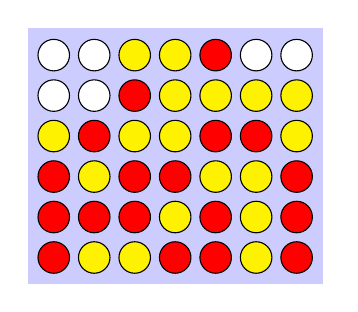
\begin{tikzpicture}%
			\fill[blue!20] (0,0) rectangle (3.75,3.25);%
			\matrix (mat) at (0,0) [matrix of nodes, ampersand replacement=\&, nodes={circle, minimum size=.4cm},%
				anchor= south west,%
			column sep={.1cm}, row sep={.1cm}] { \gy \&  \gy \&  \yw \& \yw \& \rd \&  \gy \&  \gy \&  \\
				\gy \&  \gy \&  \rd \&  \yw \& \yw \& \yw \& \yw \& \\
				\yw \& \rd \&  \yw \& \yw \& \rd \&  \rd \&  \yw \& \\
				\rd \&  \yw \& \rd \&  \rd \&  \yw \& \yw \& \rd \&  \\
				\rd \&  \rd \&  \rd \&  \yw \& \rd \&  \yw \& \rd \&  \\
				\rd \&  \yw \& \yw \& \rd \&  \rd \&  \yw \& \rd \&  \\
			};
		\end{tikzpicture}%
		\caption{As player 2}%
		\label{fig:monty}%
	\end{subfigure}%
\end{figure}%
\newpage
\section{Successor Function}
We perform two different types of ordering: static and dynamic. The static ordering is very simple. We initialize an array storing what we have determined to be an ordering that usually results in a cutoff. First we try the center, then the two columns around it, then the ones next to that, then the edges. This gives a decent performance boost because central columns are part of more winning groups than non-central edges.
		
The dynamic ordering is done using the concept of a \emph{killer heuristic}. The basic idea is that moves at the same level of the game tree are often quite similar, and what helped us prune at one node may help prune at a sibling. This is clearly the case in connect 4. Take figure \ref{fig:2} for example. If we started our search at the empty board state shown in \ref{fig:1} we would arrive at this state at a depth of 3 in our search. However we could arrive at this state in two different ways. No matter which way we use to arrive the best move choice will remain the same. By storing this best move in an array of length 42 (the number of moves possible) at index 3 (our current depth) we can make it so the next time we arrive at this state we may be able to immediately find the best choice and possibly prune the rest of the search tree by simply trying the stored best move. Although other states may be encountered between arriving at two instances of the same state, the optimal move still tends to remain the same for similar states. For example in figure \ref{fig:2}, for any placement of the second red piece (holding the central piece constant) except the central column, yellows best move is always the central column.
\begin{figure}[h]
	\centering
	\begin{subfigure}[b]{0.4\textwidth}
		\centering
		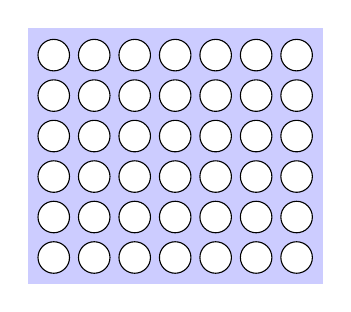
\begin{tikzpicture}
			\fill[blue!20] (0,0) rectangle (3.75,3.25);
			\matrix (mat) at (0,0) [matrix of nodes, ampersand replacement=\&, nodes={circle, minimum size=.4cm},
				anchor= south west,
			column sep={.1cm}, row sep={.1cm}] {
				\gy \& \gy \& \gy \& \gy \& \gy \& \gy \& \gy \\
				\gy \& \gy \& \gy \& \gy \& \gy \& \gy \& \gy \\
				\gy \& \gy \& \gy \& \gy \& \gy \& \gy \& \gy \\
				\gy \& \gy \& \gy \& \gy \& \gy \& \gy \& \gy \\
				\gy \& \gy \& \gy \& \gy \& \gy \& \gy \& \gy \\
				\gy \& \gy \& \gy \& \gy \& \gy \& \gy \& \gy \\
			};
		\end{tikzpicture}
		\caption{Initial state}
		\label{fig:1}
	\end{subfigure}
	\begin{subfigure}[b]{0.4\textwidth}
		\centering
		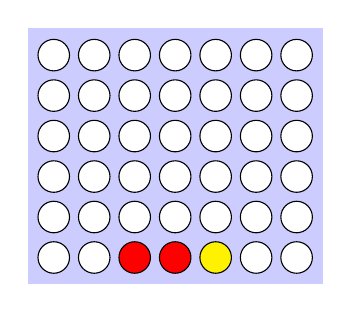
\begin{tikzpicture}
			\fill[blue!20] (0,0) rectangle (3.75,3.25);
			\matrix (mat) at (0,0) [matrix of nodes, ampersand replacement=\&, nodes={circle, minimum size=.4cm},
				anchor= south west,
			column sep={.1cm}, row sep={.1cm}] {
				\gy \& \gy \& \gy \& \gy \& \gy \& \gy \& \gy \\
				\gy \& \gy \& \gy \& \gy \& \gy \& \gy \& \gy \\
				\gy \& \gy \& \gy \& \gy \& \gy \& \gy \& \gy \\
				\gy \& \gy \& \gy \& \gy \& \gy \& \gy \& \gy \\
				\gy \& \gy \& \gy \& \gy \& \gy \& \gy \& \gy \\
				\gy \& \gy \& \rd \& \rd \& \yw \& \gy \& \gy \\
			};
		\end{tikzpicture}
		\caption{Three ply search}
		\label{fig:2}
	\end{subfigure}
		
\end{figure}	

\subsection{Abandoned Successor functions/modifications}
In addition to the scheme used, we also attempted utilizing caching to allow for quick pruning of the game tree. We set up a simple LRU cache with a limited number of entries, and tried running our alpha-beta algorithm on it for different cache sizes. Ultimately, having no cache was faster than having a cache, probably due to our poor hash generation, as we used a simple hash function that essentially just performed a bitwise and on the bitboard representing player 1 and 2, and then returned the lower 32 bits. In retrospect it is obvious why this failed, as states that fill the same slots but with different colors are extremely common in our game tree, and this would cause a very large number of colisions when retrieving from the hashtable.

There are a number of alternate hashing schemes that may have worked better, such as simply returning the long that encodes player 1's board, or extending Java's hashmap to use 64 bit keys, in which case we could encode every state as a unique 63 bit sequence (42 bits for blacks board, then 3 bits per column for the height of the column). Alternatively we could use a technique often used in chess playing AI, the Zobrist hash, which calculates a random number for each possible state of a single slot (excluding empty slots), and then loops over the board and xors the corresponding random numbers for each slot together. It may seem slow at first (we have to loop over 42 different slots initially) but the key lies in computing subsequent hashes. Since only one state has changed, we can simply xor the changed squares value with our old hash to get a new one. If we take a move back we simply xor the random value of that move, which will return the hash to its previous value. This hash function generally gives decent results.
\end{document}